\documentclass[12pt]{article}
\usepackage[english]{babel}
\usepackage{natbib}
\usepackage{url}
\usepackage[utf8x]{inputenc}
\usepackage{amsmath}
\usepackage{graphicx}
\usepackage{hyperref}
\graphicspath{{images/}}
\usepackage{parskip}
\usepackage{fancyhdr}
\usepackage{listings}
\usepackage{hyperref}
\usepackage{color}

\definecolor{codegreen}{rgb}{0,0.6,0}
\definecolor{codegray}{rgb}{0.5,0.5,0.5}
\definecolor{codepurple}{rgb}{0.58,0,0.82}
\definecolor{backcolour}{rgb}{0.95,0.95,0.92}

\lstdefinestyle{mystyle}{
    backgroundcolor=\color{backcolour},   
    commentstyle=\color{codegreen},
    keywordstyle=\color{magenta},
    numberstyle=\tiny\color{codegray},
    stringstyle=\color{codepurple},
    basicstyle=\ttfamily\footnotesize,
    breakatwhitespace=false,         
    breaklines=true,                 
    captionpos=b,                    
    keepspaces=true,                 
    numbers=left,                    
    numbersep=5pt,                  
    showspaces=false,                
    showstringspaces=false,
    showtabs=false,                  
    tabsize=2
}

\lstset{style=mystyle}
\renewcommand{\lstlistingname}{Snippet}
\renewcommand{\lstlistlistingname}{Snippets}
\def\lstlistingautorefname{Snippet}



\hypersetup{
    colorlinks=true,    % Enable colored links instead of boxed links
    linkcolor=black,     % Color for internal links (sections, pages)
    urlcolor=black,      % Color for external URLs
    citecolor=black,     % Color for citation links
    filecolor=black   % Color for file links
}
%\usepackage{vmargin}
%\setmarginsrb{2 cm}{2.5 cm}{3 cm}{2.5 cm}{1 cm}{1.5 cm}{1 cm}{1.5 cm}

\topmargin=-0.2in    
\textheight=9in     %24.1cm
\evensidemargin=0in %0cm
\oddsidemargin=0in  %-.3cm
\textwidth=6.5in    %16.5cm

\title{Assignment Name \\ about \\ \vspace{0.5cm} Subject}								% Title
\author{Author Name}								% Author
\date{\today}											% Date

\makeatletter
\let\thetitle\@title
\let\theauthor\@author
\let\thedate\@date
\makeatother

\pagestyle{fancy}
\fancyhf{}
\rhead{\theauthor}
\lhead{School of Computing}
\rfoot{\thepage}

\begin{document}
\vspace{-2cm}
%%%%%%%%%%%%%%%%%%%%%%%%%%%%%%%%%%%%%%%%%%%%%%%%%%%%%%%%%%%%%%%%%%%%%%%%%%%%%%%%%%%%%%%%%

\begin{titlepage}
	\centering
    %\vspace*{0.1 cm}
    
\includegraphics[scale = 1]{logo.png}\\[1.0 cm]	% University Logo
    \textsc{\LARGE The Knowledge Hub \\ \vspace{0.5cm} Universities}\\[1.5 cm]	% University Name
	\textsc{\Large KH00000XXX}\\[0.5 cm]				% Course Code
	\textsc{\large Module Name}\\[0.5 cm]				% Course Name
	\rule{\linewidth}{0.2 mm} \\[0.4 cm]
	{ \huge \bfseries \thetitle}\\
	\rule{\linewidth}{0.2 mm} \\[1.5 cm]
	
    {\large \thedate}\\[1 cm]
    
	\begin{minipage}{0.4\textwidth}
		\begin{flushleft} \large
			\emph{Author:}\\
			\theauthor
			\end{flushleft}
			\end{minipage}~
			\begin{minipage}{0.4\textwidth}
			\begin{flushright} \large
			\emph{Student ID:} \\
			CU0000000									% Your Student Number
		\end{flushright}
	\end{minipage}\\
	
	
 
	\vfill
	
\end{titlepage}

%%%%%%%%%%%%%%%%%%%%%%%%%%%%%%%%%%%%%%%%%%%%%%%%%%%%%%%%%%%%%%%%%%%%%%%%%%%%%%%%%%%%%%%%%
\pagenumbering{gobble}
\tableofcontents
\pagebreak

\flushbottom


% IF YOU WANT A LIST OF TABLE AND LIST OF FIGURES UNCOMMENT THE LINES DOWN HERE
% \pagenumbering{gobble}
% \listoffigures
% \listoftables
% \newpage


%%%%%%%%%%%%%%%%%%%%%%%%%%%%%%%%%%%%%%%%%%%%%%%%%%%%%%%%%%%%%%%%%%%%%%%%%%%%%%%%%%%%%%%%%
\pagenumbering{arabic}
\section{Introduction}
Here is text in bold \textbf{consectetur adipiscing elit, sed do eiusmod tempor incididunt ut labore et dolore magna aliqua}. Here's text in italic. \textit{Duis aute irure dolor in reprehenderit in voluptate velit esse cillum dolore eu fugiat nulla pariatur}. Here are references \cite{zeng2010} and \cite{wang2007}, and finally \citep{harris2009}.

\section{Section 1}
References are stored in a Bibtex file. Google Scholar and IEEExplore allow you to download citations of papers in Bibtex format from their search engine. Some people use JabRef (\url{http://www.jabref.org}) to manage their reference database.

This is an inline equation $\Gamma(t)=K_i e^{\sin^2(\omega_t)}$. The first paragraph appears without indent but the following ones will have an indentation.

This is an actual named equation:
\begin{equation}
v(x)=\frac{1}{2}\sin(2 \omega t + \phi) e^{-j s t}
\label{eq:cacona}
\end{equation}
\noindent where $\omega$ is the angular speed. We can reference the equation like this (\ref{eq:cacona}). \LaTeX\ is pretty good at mathematical notations, so I suggest you look that up.



\subsection{Subsection 1}
This is what happens when we have multiple subsections. This is the first one.

\paragraph{Paragraph example}
Here's how you could differentiate paragraphs:\\
Lorem ipsum dolor sit amet, consectetur adipiscing elit, sed do eiusmod tempor incididunt ut labore et dolore magna aliqua. Ut enim ad minim veniam, quis nostrud exercitation ullamco laboris nisi ut aliquip ex ea commodo consequat. Duis aute irure dolor in reprehenderit in voluptate velit esse cillum dolore eu fugiat nulla pariatur. Excepteur sint occaecat cupidatat non proident, sunt in culpa qui officia deserunt mollit anim id est laborum, 

\subsection{Subsection 2}


We can reference a table like this Table~\ref{tab:tab1}. A figure is shown Fig~\ref{fig:fig1}, we don't necessarily know if this figure will appear below, above or elsewhere; therefore, the text should never refer to the figure with sentences such as {\it "As shown here:"}.


\begin{table}[htbp]
	\centering
	\begin{tabular}{lll}
		Thing 1 & Thing 2 & Thing 3\\
		\hline
		$x$ & 1 & x \\
		$y$ & 0 & y\\
	    \hline
	\end{tabular}
	\caption{How to do a table}
	\label{tab:tab1}
\end{table}

\subsubsection{Sub-Subjection}
Sometimes, We can add footnotes to something \footnote{Like this example.}. Here's another type of table.\\
\begin{table}[ht]
\center
\begin{tabular}{c|c|c}
A & B & A XOR B\\
\hline
0 & 0 & 0\\
0 & 1 & 1\\
1 & 0 & 1\\
1 & 1 & 0\\
\end{tabular}
\caption{A simple table in \LaTeX.}
\label{tab:xor}
\end{table}


\section{Section 2}
We can also easily add figures and stuff.

\begin{figure}[htbp]
	\centering
        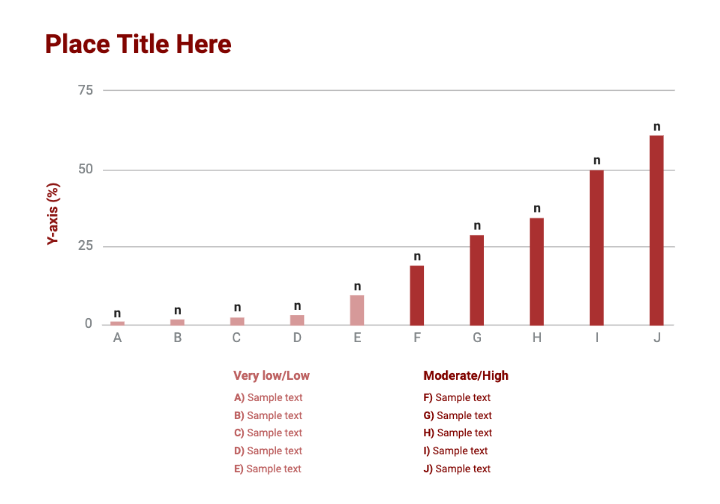
\includegraphics[scale = 0.6]{Figure1.png}\\[1.0 cm]
	\caption{How to do a figure.}
	\label{fig:fig1}
\end{figure}



You can even put code snippets. You can use the \lstinline|print()| function to display the output in Python. Or you can use larger code blocks:
\begin{lstlisting}[language=Python, caption=Sample Python Code, label=lst:sample_python]
def hello_world():
    print("Hello, world!")
\end{lstlisting}

\section{Conclusion}
You can do a lot with this and I recommend that you further research it to make quality reports. Don't forget to check out the references in the next page. It displays is automatically.

%\hspace{1 cm}--- Linus

\newpage
% \bibliographystyle{apalike}
\bibliographystyle{unsrt}
\bibliography{biblist}

\end{document}